\documentclass[epsfig,10pt,fullpage]{article}

\newcommand{\LabNum}{5}
\newcommand{\CommonDocsPath}{../../common/docs}
\addtolength{\textwidth}{1.5in}
\addtolength{\oddsidemargin}{-0.75in}
\addtolength{\topmargin}{-0.75in}
\addtolength{\textheight}{1.5in}
\addtolength{\evensidemargin}{0.75in}
\setlength\parindent{0pt}
\raggedbottom

\usepackage{ae,aecompl}
\usepackage{epsfig,float,times}
\usepackage[hypcap]{caption}
\usepackage[pdftex, colorlinks]{hyperref}
\usepackage{graphicx}
\usepackage[usenames, dvipsnames]{color}
\usepackage{rotating}
\usepackage{tikz}
\usetikzlibrary{automata,positioning}
\usepackage{placeins}

\widowpenalty 10000
\clubpenalty 10000

\newcommand{\red}[1]{{\color{red}\sf{#1}}}
\newcommand{\green}[1]{{\color{green}\sf{#1}}}
\newcommand{\blue}[1]{{\color{blue}\sf{#1}}}
\definecolor{PineGreen}{rgb}{0.0, 0.47, 0.44}
\definecolor{ForestGreen}{rgb}{0.13, 0.55, 0.13}
\definecolor{Brown}{rgb}{0.59, 0.29, 0.0}

\newcommand{\UPDatePublished}{Oct 2021}
\newcommand{\versnum}{21.1} %version number quartus/AMP
\newcommand{\quartusname}{Quartus\textsuperscript{\textregistered} Prime}	
\newcommand{\UPTextBar}{For \quartusname{} \versnum{}}
\newcommand{\thisyear}{2021 } %for copyright
\newcommand{\company}{FPGAcademy.org}
\newcommand{\longteamname}{FPGAcademy.org}
\newcommand{\teamname}{FPGAcademy}
\newcommand{\website}{FPGAcademy.org}

\newcommand{\productAcronym}{AMP}
\newcommand{\productNameShort}{Monitor Program}

\newcommand{\productNameMedTM}{A Monitor Program}
\newcommand{\productNameMed}{A Monitor Program}

%\newcommand{\headerLogoFilePath}[1]{#1/FPGAcademy.png}

% listings is a package that supports encapsulating source code in LaTeX conveniently
\usepackage{listings}

\def\expandparam\lstinputlisting[#1]#2{\edef\tmp{\noexpand\lstinputlisting[#1]{#2}}\tmp}

%%%%%%%%%%%%%%%%%%%% Source Code Formatting %%%%%%%%%%%%%%%%%%%%
\definecolor{globalCommentColour}{rgb}{0.588,0.588,0.588}

%%%%%%%%%%%%%%%%%%%%%%%%%%%%%%%%%%%%%%%%%%%%%%%%%%%%
% Defining language style
% NiosII ASM
\lstdefinelanguage[NiosII]{Assembler} {
  morekeywords={add, addi, and, andhi, andi, beq, bge, bgeu, bgt, bgtu, ble,  bleu, blt, bltu, bne, br, break,
  bret, call, callr, cmpeq, cmpeqi, cmpge, cmpgei, cmpgeu, cmpgeui, cmpgt, cmpgti, cmpgtu, cmpgtui, cmple,
  cmplei, cmpleu, cmpleui, cmplt, cmplti, cmpltu, cmpltui, cmpne, cmpnei, custom, div, divu, eret, flushd,
  flushda, flushi, flushp, initd, initda, initi, jmp, jmpi, ldb, ldbio, ldbu, ldbuio, ldh, ldhio, ldhu, ldhuio,
  ldw, ldwio, mov, movhi, movi, movia, movui, mul, muli, mulxss, mulxsu, mulxuu, nextpc, nop, nor, or, orhi, ori,
  rdctl, rdprs, ret, rol, roli, ror, sll, slli, sra, srai, srl, srli, stb, stbio, sth, sthio, stw, stwio,
  sub, subi, sync, trap, wrctl, wrtcl, wrprs, xor, xori, xorhi, xori},
  morekeywords=[2]{.abort, .ABORT, .align, .app-file, .ascii, .asciz, .balign, .byte, .comm, .data, .def,
  .desc, .dim, .double, .eject, .else, .end, .endef, .endif, .equ, .equiv, .err, .extern, .file, .fill, .float,
  .global, .globl, .hword, .ident, .if, .include, .int, .irp, .irpc, .lcomm, .lflags, .line, .linkonce, .ln,
  .list, .long, .macro, .mri, .nolist, .octa, .org, .p2align, .psize, .quad, .rept, .sbttl, .scl, .section,
  .set, .short, .single, .size, .sleb128, .skip, .space, .stadb, .stabn, .stabs, .string, .symver, .tag,
  .text, .title, .type, .val, .uleb128, .word},
  morekeywords=[3]{et, bt, gp, sp, fp, ea, sstatus, ra, pc, status, estatus, bstatus, ienable, ipending, cpuid,
  exception, pteaddr, tlbacc, tlbmisc, eccinj, badaddr, config, mpubase, mpuacc},
  sensitive=t,
  alsoletter=.,
  morestring=[b]",
  morecomment=[s]{/*}{*/},
  morecomment=[l]\#,
}[keywords,comments,strings]
   
%% NOTE: morekeywords=[2] are GNU directives.
   
\definecolor{niosInstructionColour}{rgb}{0.000,0.608,0.000}
\definecolor{niosDirectiveColour}{rgb}{0.000,0.000,0.902}
\definecolor{niosSpecialRegColour}{rgb}{0.000,0.000,0.000}
\definecolor{niosStringColour}{rgb}{0.808,0.482,0.000}
   
%% NOTE: To make bold use: =\bfseries\color{<colour>}
\lstdefinestyle{defaultNiosStyle} {
  language=[NiosII]{Assembler},
  stringstyle=\color{niosStringColour},
  keywordstyle=\color{niosInstructionColour},
  keywordstyle=[2]\color{niosDirectiveColour},
  keywordstyle=[3]\itshape\color{niosSpecialRegColour}
}
%%%%%%%%%%%%%%%%%%%%%%%%%%%%%%%%%%%%%%%%%%%%%%%%%%%%

%%%%%%%%%%%%%%%%%%%%%%%%%%%%%%%%%%%%%%%%%%%%%%%%%%%%
% Defining language style
% ArmA9 ASM
\lstdefinelanguage[ArmA9]{Assembler} {
  morekeywords={ADC, ADD, ADDS, AND, ANDS, B, BAL, BEQ, BGE, BGT, BL, BLT, BIC, BKPT, BLX, BNE, BX, CDP, CLZ, CMN, CMP, EOR,
  EORS, LDC, LDM, LDR, LDRB, LDRBT, LDRH, LDRSB, LDRSH, LDRT, LSL, MCR, MLA, MOV, MOVW, MOVT, MRC, MRS, MSR, MUL, MVN, ORR, PLD,
  ROR, RSB, RSC, SBC, SMLAL, SMULL, STC, STM, STR, STRB, STRBT, STRH, STRT, SUB, SUBS, SWI, SWP, SWPB, TEQ, UMLAL,
  PUSH, POP, MOVS, RORS, LSR},
  morekeywords=[2]{.abort, .ABORT, .align, .app-file, .ascii, .asciz, .balign, .byte, .comm, .data, .def,
  .desc, .dim, .double, .eject, .else, .end, .endef, .endif, .equ, .equiv, .err, .extern, .file, .fill, .float,
  .global, .globl, .hword, .ident, .if, .include, .int, .irp, .irpc, .lcomm, .lflags, .line, .linkonce, .ln,
  .list, .long, .macro, .mri, .nolist, .octa, .org, .p2align, .psize, .quad, .rept, .sbttl, .scl, .section,
  .set, .short, .single, .size, .sleb128, .skip, .space, .stadb, .stabn, .stabs, .string, .symver, .tag,
  .text, .title, .type, .val, .vectors, .uleb128, .word},
  morekeywords=[3]{SP, PC, MIDR, CTR, TCMTR, TLBTR, MPIDR, ID_PFR0, ID_PFR1, ID_DFR0, ID_MMFR0, ID_MMFR1, ID_MMFR2,
  ID_MMFR3, ID_ISAR0, ID_ISAR1, ID_ISAR2, ID_ISAR3, ID_ISAR4, CCSIDR, CLIDR, AIDR, CSSELR, TTBR0, TTRB1, TTBR2, DACR,
  DFSR, IFSR, ADFSR, AIFSR, DFAAR, IFAR, ICIALLUIS, BPIALLIS, PAR, ICIALLU, ICIMVAU, BPIALL, DCIMVAC, DCISW, V2PCWPR,
  DCCVAC, DCCSW, DDIMVAC, DCISW, TLBALLIS, TLBIMVAIS, TLBIASIDIS, TLBIMVAAIS, TLBIALL, TLBIMVA, TLBIASID, TLBIMVAA,
  PMCR, PMCNTENSET, PMCNTENCLR, PMOVSR, PMSWINC, PMSELR, PMXEVTYPER, PMXEVCNTR, PMUSERENR, PMINTENSET, PMINTENCLR,
  PRRR, NRRR, PLEIDR, PLEASR, PLEFSR, PLEUAR, PLEPCR, VBAR, MVBAR, ISR, FCSEIDR, CONTEXTIDR, TPIDRURW, TPIDRURO, TPIDRPRW},
  sensitive=f,
  alsoletter=.,
  morestring=[b]",
  morecomment=[s]{/*}{*/},
  morecomment=[l]{//},
}[keywords,comments,strings]
   
%% NOTE: morekeywords=[2] are GNU directives.
   
\definecolor{armInstructionColour}{rgb}{0.000,0.608,0.000}
\definecolor{armDirectiveColour}{rgb}{0.000,0.000,0.902}
\definecolor{armSpecialRegColour}{rgb}{0.000,0.000,0.000}
\definecolor{armStringColour}{rgb}{0.808,0.482,0.000}
   
\lstdefinestyle{defaultArmStyle} {
  language=[ArmA9]{Assembler},
  stringstyle=\color{armStringColour},
  keywordstyle=\color{armInstructionColour},
  keywordstyle=[2]\color{armDirectiveColour},
  keywordstyle=[3]\itshape\color{armSpecialRegColour}
}
%%%%%%%%%%%%%%%%%%%%%%%%%%%%%%%%%%%%%%%%%%%%%%%%%%%%

%%%%%%%%%%%%%%%%%%%%%%%%%%%%%%%%%%%%%%%%%%%%%%%%%%%%
% Defining language style
% FPGAcademy ASM
\lstdefinelanguage{ASM}{
  morekeywords = [1]{mv, mvt, mvne, mvcc, add, sub, st, ld, and, b, bne, beq, bcc, bcs},
  morekeywords = [2]{word, define},
  keywordstyle = [1]\color{ForestGreen},
  keywordstyle = [2]\color{blue},
  sensitive = true,
  morecomment = [l]{//},
}

\lstset{
  language = ASM,
  basicstyle=\small\color{black}\ttfamily,
  commentstyle=\small\color{Brown}\itshape\ttfamily,
  showstringspaces=false,
  frame=none, %lines % boxed listings
  breaklines=true,
  breakatwhitespace=true,
  tabsize=3
}
%%%%%%%%%%%%%%%%%%%%%%%%%%%%%%%%%%%%%%%%%%%%%%%%%%%%

%%%%%%%%%%%%%%%%%%%%%%%%%%%%%%%%%%%%%%%%%%%%%%%%%%%%
% Defining language style
% Java
\definecolor{javaStringColour}{rgb}{0.808,0.482,0}
%%%%%%%%%%%%%%%%%%%%%%%%%%%%%%%%%%%%%%%%%%%%%%%%%%%%

%%%%%%%%%%%%%%%%%%%%%%%%%%%%%%%%%%%%%%%%%%%%%%%%%%%%
% Defining language style
% C
\definecolor{CStringColour}{rgb}{0.808,0.482,0}

\lstset{
  language = C,
  basicstyle=\small\color{black}\ttfamily, 
  commentstyle=\small\color{PineGreen}\itshape\ttfamily,
  keywordstyle=\small\color{blue}\bfseries\ttfamily,
  showstringspaces=false,
  frame=none, %lines % boxed listings
  breaklines=true,
  breakatwhitespace=true,
  tabsize=3
}
%%%%%%%%%%%%%%%%%%%%%%%%%%%%%%%%%%%%%%%%%%%%%%%%%%%%

%%%%%%%%%%%%%%%%%%%%%%%%%%%%%%%%%%%%%%%%%%%%%%%%%%%%
% Defining language style
% Verilog
\definecolor{verilogCommentColour}{rgb}{0.000,0.502,0.000}

\lstdefinestyle{defaultVerilogStyle} {
  language={Verilog},
  keywordstyle=\color{blue},
  commentstyle=\color{verilogCommentColour}
}
%%%%%%%%%%%%%%%%%%%%%%%%%%%%%%%%%%%%%%%%%%%%%%%%%%%%

%%%%%%%%%%%%%%%%%%%%%%%%%%%%%%%%%%%%%%%%%%%%%%%%%%%%
% Defining language style
% VHDL
\lstdefinestyle{defaultVHDLStyle} {
  language={VHDL},
  keywordstyle=\color{blue},
  commentstyle=\color{verilogCommentColour}
}
%%%%%%%%%%%%%%%%%%%%%%%%%%%%%%%%%%%%%%%%%%%%%%%%%%%%

%%%%%%%%%%%%%%%%%%%%%%%%%%%%%%%%%%%%%%%%%%%%%%%%%%%%
% Defining language style
% LaTeX
\lstdefinelanguage[LocalLaTeX]{TeX}[LaTeX]{TeX}{moretexcs={bf, it, sf, lstset},}

\lstdefinestyle{defaultLocalLatexStyle} {
  language=[LocalLatex]{TeX},
  keywordstyle=\color{blue}\bfseries,
  keywordstyle=[2]\color{blue},
  keywordstyle=[3]\color{blue}\bfseries
}
%%%%%%%%%%%%%%%%%%%%%%%%%%%%%%%%%%%%%%%%%%%%%%%%%%%%

%%%%%%%%%%%%%%%%%%%%%%%%%%%%%%%%%%%%%%%%%%%%%%%%%%%%
% Defining language style
% Default
\lstset{
  basicstyle=\small\color{black}\ttfamily,
  commentstyle=\small\color{globalCommentColour}\itshape\ttfamily,
  keywordstyle=\small\color{blue}\bfseries\ttfamily,
  showstringspaces=false,
  frame=none, %lines % boxed listings
  breaklines=true,
  breakatwhitespace=true,
  tabsize=3
}
%%%%%%%%%%%%%%%%%%%%%%%%%%%%%%%%%%%%%%%%%%%%%%%%%%%%


\hypersetup{
  pdftitle={Embedded Systems Lab Exercise \LabNum},
  linkcolor=blue,
  hyperindex=true,
  pdfauthor={FPGAcademy.org},
  pdfkeywords={FPGAcademy.org, FPGAcademy, Lab, Exercise, Embedded Systems},
  bookmarks,
  bookmarksopen=false,
  filecolor=blue,
  pdfstartview={FitH},
  urlcolor=blue,
  plainpages=false,
  pdfpagelabels=true,
  linkbordercolor={1 1 1} %no color for link border
}



\begin{document}

\centerline{\huge Embedded Systems}
~\\
\centerline{\huge Laboratory Exercise \LabNum}
~\\
\centerline{\large Using ASCII Graphics for Animation}
~\\

\noindent
The purpose of this exercise is to learn how to perform simple animations under Linux*. 
Graphics will be ``drawn'' by sending ASCII {\it escape commands} to the Linux Terminal window.
We assume that the reader is using the DE1-SoC, DE10-Standard, or DE10-Nano board.

\noindent
\section*{Part I}

\noindent
Although a Linux Terminal window normally displays ASCII text, we can use the 
Terminal's {\it escape command} sequences to make simple drawings, often called 
{\it ASCII graphics}. Animations can be created on the Terminal by using commands to 
clear the screen, move the Terminal cursor to specific locations, show/hide the cursor, 
change the color of characters, and so on. An example of a program that uses ASCII graphics is 
given in Figure~\ref{fig:dots}. 

\lstset{language=C,numbers=left,escapechar=|}
\begin{figure}[h]
\begin{center}
\begin{minipage}[t]{12.5 cm}
\begin{lstlisting}[name=dots]
|\label{line:includes}|/* This program draws a few characters on the screen. */
#include <stdio.h>
#define YELLOW 33
#define CYAN 36
#define WHITE 37

void plot_pixel(int, int, char, char);

int main(void) {
	char c;
	int i;
	|\label{line:clear}|printf ("\e[2J"); 				// clear the screen
  	|\label{line:hide}|printf ("\e[?25l");				// hide the cursor

	|\label{line:plot1}|plot_pixel (1, 1, CYAN, 'X');
	plot_pixel (80, 24, CYAN, 'X');
	for (i = 8; i < 18; ++i)
	   |\label{line:plot2}|plot_pixel (40, i + 12, YELLOW, '*');

	|\label{line:getchar}|c = getchar ();					// wait for user to press return
	printf ("\e[2J"); 				// clear the screen
	|\label{line:reset}|printf ("\e[%2dm", WHITE);		// reset foreground color
	|\label{line:cursor}|printf ("\e[%d;%dH", 1, 1);	// move cursor to upper left
	|\label{line:show}|printf ("\e[?25h");				// show the cursor
	|\label{line:fflush}|fflush (stdout);
}

|\label{line:pp1}|void plot_pixel(int x, int y, char color, char c)
{
  	|\label{line:pixel}|printf ("\e[%2dm\e[%d;%dH%c", color, y, x, c);
  	fflush (stdout);
|\label{line:pp2}|}
\end{lstlisting}
\end{minipage}
\caption{An example of code that uses ASCII graphics.}
\label{fig:dots}
\end{center}
\end{figure}

\noindent
The first line of code in Figure~\ref{fig:dots} {\it includes} 
the {\it stdio.h} library, which is required to use the {\it printf} function. The next three 
lines define constants, described later, for text colors which can be used in the Terminal window. 
A command is sent to the Terminal in line~\ref{line:clear} by using {\it printf}. All Terminal 
window commands begin with the ASCII \texttt{ESC} (escape) character, which is specified 
in the {\it printf} string using the syntax $\backslash$e. The command in line~\ref{line:clear},
which is \texttt{[2J}, instructs the Terminal to clear the screen. Another command, 
\texttt{[?25l}, given in line~\ref{line:hide}, causes the Terminal to {\it hide} the cursor 
so that it is not visible to the user. Next, the function \texttt{plot\_pixel} is called to draw
some characters at specific locations on the screen. In this example the size of the Terminal 
window is assumed to be 80 columns by 24 rows. Coordinates $(1, 1)$ are at the top-left corner 
of the screen and $(80, 24)$ are at the bottom-right corner. The calls to \texttt{plot\_pixel} in
lines~\ref{line:plot1} to~\ref{line:plot2} draw cyan-colored \texttt{X} characters at
coordinates ($1, 1$) and ($80, 24$), and a vertical yellow line of ten \texttt{*} characters
down the middle of the screen.

~\\
\noindent The \texttt{plot\_pixel} function, shown in lines~\ref{line:pp1} to~\ref{line:pp2} uses 
two commands to draw a character. The first command is \texttt{[ccm}, where $cc$ is
called an {\it attribute}. The attribute can be used to set the color of text characters,
by using different values of $cc$. Examples of color attributes are $cc = 31$ (red), 
32 (green), 33 (yellow), 34 (blue), 35 (magenta), 36 (cyan), and 37 (white). The second command 
in \texttt{plot\_pixel} is \texttt{[yy;xxH}, where $yy$ and $xx$ specify a row and
column on the screen, respectively. This command moves the Terminal cursor to $(x,y)$ coordinates
$(xx, yy)$. In line~\ref{line:getchar} the program waits, using the \texttt{getchar}
function, for the user to press a key. Finally, commands are sent to the Terminal to {\it clear} 
the screen, {\it set} the color to white, {\it set} the cursor to coordinates ($1, 1$), and
{\it show} the cursor.

~\\
\noindent 
The use of ASCII graphics described above became popular around the year 1980 when they
were available in computer video terminals called the {\it VT100}, manufactured by Digital 
Equipment Corporation. The Linux Terminal provides ASCII graphics by {\it emulating} the 
capabilites of the VT100 video terminal. A listing of some escape commands is given in 
a table at the end of this document. More information about ASCII graphics 
commands can be found by searching on the Internet for a topic such as ``VT100 graphics''.

~\\
\noindent
Perform the following

\begin{enumerate}

\item Create a C source-code file for Figure~\ref{fig:dots}. The code is provided along 
with this laboratory exercise.

\item Compile your program and execute it in a Linux Terminal window to display the ASCII
graphics.

\end{enumerate}

\noindent
\section*{Part II}

\noindent
In this part you will learn how to implement a simple line-drawing algorithm.

~\\
\noindent
Drawing a line on a screen requires coloring ``pixels'' between two coordinates $(x_1,y_1)$ and 
$(x_2,y_2)$, such that the pixels represent the desired line as closely as possible. In
the case of ASCII graphics, a {\it pixel} represents a character coordinate on the screen.
Consider the example in Figure~\ref{fig:line_drawing}, where we want to draw a line between 
coordinates $(1,1)$ and $(12,5)$. The squares in the figure represent the location and 
size of pixels on the screen. As indicated in the figure, we cannot draw the line 
precisely---we can only draw a shape that is similar to the line by coloring the pixels that 
fall closest to the line's ideal location on the screen.

\begin{figure}[h]
   \begin{center}
			  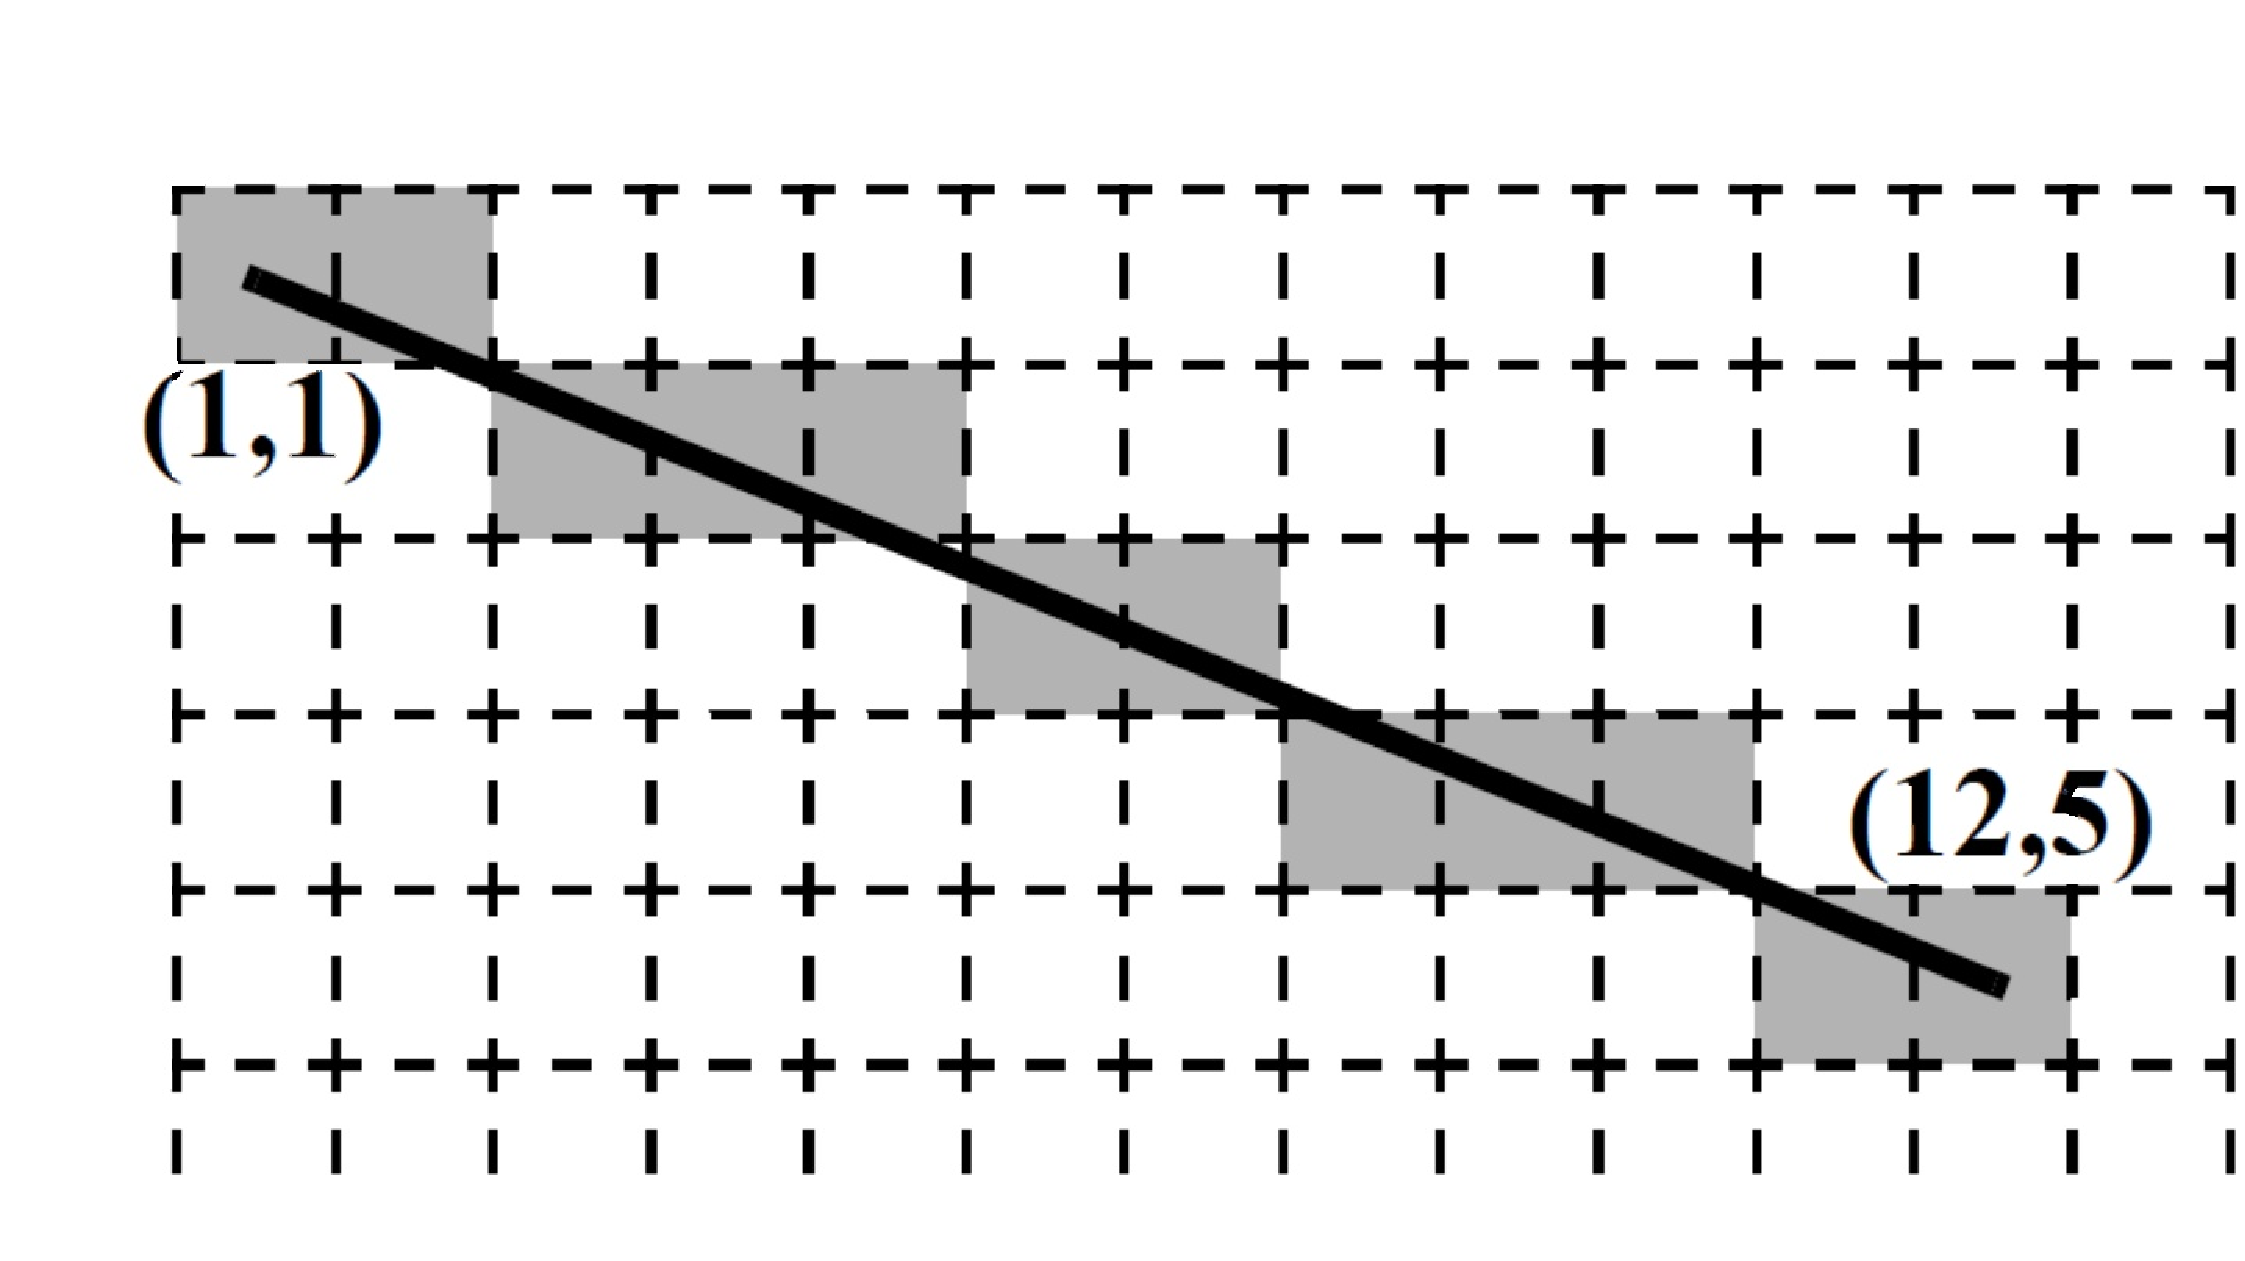
\includegraphics[width=6cm]{figures/fig_line_drawing_vt100}
   \end{center}
   \caption{Drawing a line between coordinates $(1,1)$ and $(12,5)$.}
	\label{fig:line_drawing}
\end{figure}

~\\
\noindent
We can use algebra to determine which pixels to color. This is done by using the end points and 
the slope of the line. The slope of our example line is $slope = (y_2 - y_1)/(x_2 - x_1) = 4/11$. 
Starting at point $(1,1)$ we move along the $x$ axis and compute the $y$ coordinate for the 
line as follows:

\begin{eqnarray*}
y = y_1 + slope \times (x - x_1)
\end{eqnarray*}

~\\
\noindent
Thus, for column $x = 2$, the $y$ location of the pixel is
$1 + \frac{4}{11} \times (2-1) = 1 \frac{4}{11}$. 
Since pixel locations are defined by integer values we round the $y$ coordinate to the nearest 
integer, and determine that in column $x = 2$ we should color the pixel at $y = 1$. For
column $x = 3$ we perform the calculation $y = 1 + \frac{4}{11} \times (3-1) = 1
\frac{8}{11}$, and round the result to $y = 2$.  Similarly, we perform such computations 
for each column between $x_1$ and $x_2$.

\noindent
The approach of moving along the $x$ axis has drawbacks when a line is steep. A steep line
spans more rows than it does columns, and hence has a slope with absolute value greater than~1.
In this case our calculations will not produce a smooth-looking line.  Also, in the case
of a vertical line we cannot use the slope to make a calculation.  To address this 
problem, we can alter the algorithm to move along the $y$ axis when a line is steep. With 
this change, we can implement a line-drawing algorithm known as {\it Bresenham's algorithm}.
A key property of this algorithm is that all variables are {\it integers}.
Pseudo-code for this algorithm is given in Figure~\ref{fig:bresenham}. The first~\ref{line:adjust}
lines of the algorithm make the needed adjustments depending on whether or not the line is
steep, and to account for the horizontal and vertical directions of the line. 
Then, in lines~\ref{line:f1} to~\ref{line:f2} the algorithm increments the 
{\it x} variable 1 step at a time
and computes the {\it y} value. The {\it y} value is incremented when needed to stay as
close to the ideal location of the line as possible. Bresenham's algorithm calculates an
{\it error} variable to decide whether or not to increment each {\it y} value. 
The {\it error} variable takes into account the relative difference
between the width of the line ({\it deltax}) and height of the line ({\it deltay}) in deciding
how often {\it y} should be incremented. The version of the algorithm shown in 
Figure~\ref{fig:bresenham} uses only integers to perform all calculations. 

\begin{figure}[h]
\begin{center}
\begin{minipage}[t]{12.5 cm}
\begin{lstlisting}[name=bresenham]
draw_line(x0, x1, y0, y1)

	is_steep = (abs(y1 - y0) > abs(x1 - x0))
	if is_steep then
		swap(x0, y0)
		swap(x1, y1)
	if x0 > x1 then
		swap(x0, x1)
		swap(y0, y1)

	deltax = x1 - x0
	deltay = abs(y1 - y0)
	error = -(deltax / 2)
	y = y0
	|\label{line:adjust}|if y0 < y1 then y_step = 1 else y_step = -1

	|\label{line:f1}|for x from x0 to x1
		if is_steep then draw_pixel(y,x) else draw_pixel(x,y)
		error = error + deltay
		if error |$\ge$| 0 then
			y = y + y_step
			|\label{line:f2}|error = error - deltax
\end{lstlisting}
\end{minipage}
\caption{Pseudo-code for a line-drawing algorithm.}
\label{fig:bresenham}
\end{center}
\end{figure}

\noindent
Perform the following:

\begin{enumerate}

\item Write a C program that uses Bresenham's line-drawing algorithm to draw a few lines on 
the screen.  An example of output that your program might produce is illustrated in 
Figure~\ref{fig:lines}. In this example the lines are drawn using the `*' character, but
you can use any ASCII character to draw your lines.

\item Compile and test your program using a Linux Terminal.

\end{enumerate}

\begin{figure}[h]
   \begin{center}
			  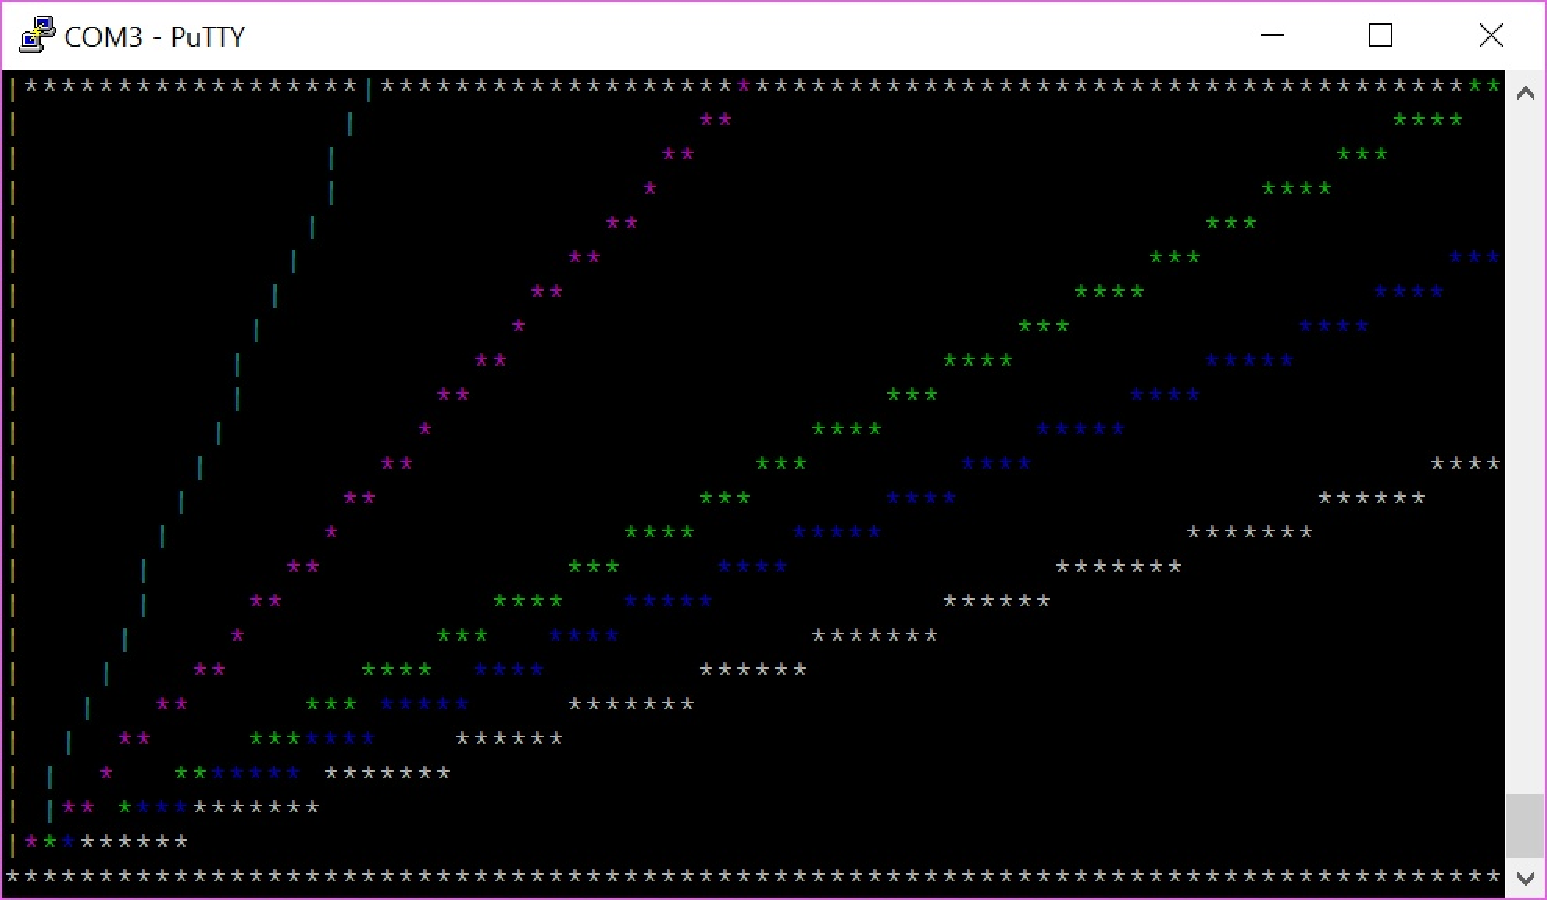
\includegraphics[width=12cm]{figures/lines}
   \end{center}
   \caption{Drawing a few lines on the screen.}
	\label{fig:lines}
\end{figure}

\newpage
\noindent
\section*{Part III}

\noindent
Animation is an exciting part of computer graphics. Moving a displayed object is an illusion 
created by showing this same object at different locations on the screen. A simple way to
``move'' an object is to first draw the object at one position, and then after a short time erase 
the object and draw it again at another nearby position.

~\\
\noindent
To realize animation it is necessary to move objects at regular time intervals. For this
exercise we can use a timer controlled by the Linux kernel, such as the {\it nanosleep}
function. A reasonable delay might be about $0.1$ seconds, but you should experiment with 
different animation delays and observe the results. Documentation for {\it nanosleep} can be 
obtained by searching on the Internet.

~\\
\noindent
Perform the following:

\begin{enumerate}

\item Write a C-language program that moves a horizontal line up and down on the screen and 
``bounces'' the line off the top and bottom edges of the display. Your program should first 
clear the screen and then draw the line at a starting row. Then, in an endless loop you should
erase the line, and redraw it one row above or below the last one. When the line reaches the 
top, or bottom, of the screen it should start moving in the opposite direction. Note that
the Terminal window may be somewhat {\it slow} to receive ASCII characters, and this may
limit the speed of your animation. When erasing a line, it may be more efficient to clear the
whole screen, using the escape command \texttt{[2J}, as compared to redrawing the line by
printing black characters.

\item Compile your code and test it. Experiment with different animation delay times.
\end{enumerate}
\noindent
\section*{Part IV}

\noindent
Having gained some basic knowledge about drawing lines and animations, you can now create 
a more interesting animation.

~\\
\noindent
You are to create an animation of several objects on the screen. These objects should appear 
to be moving continuously and ``bouncing'' off the edges of the screen. The objects should 
be connected with lines to form a chain. An illustration of the animation is given in 
Figure~\ref{fig:animation_example}. Part $a$ of the figure shows one position
of the objects with arrows that indicate the directions of movement, and 
Figure~\ref{fig:animation_example}$b$ shows a subsequent position of the objects. 
In each step of your animation each of the objects should appear to ``move'' on a diagonal 
line: up/left, up/right, down/left, or down/right. Move the objects one row and one column 
at a time on the Terminal screen.

\begin{figure}[h!]
   \begin{center}
       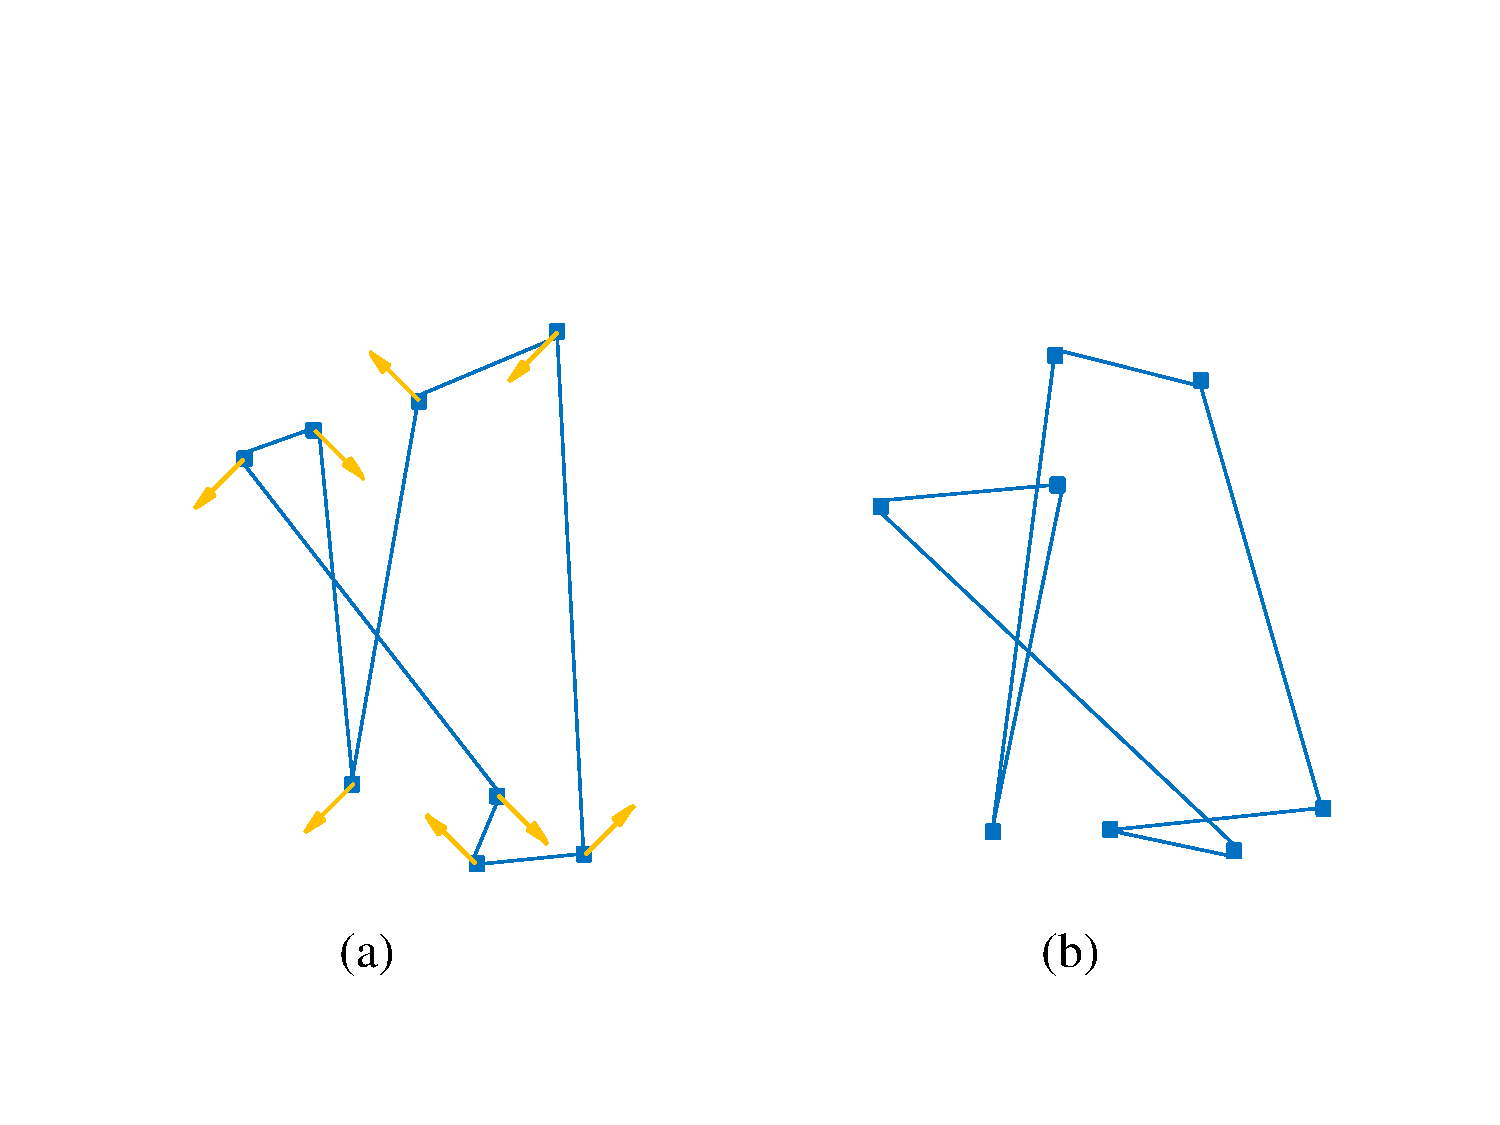
\includegraphics[scale = 0.5]{figures/fig_animation_example.pdf}
   \end{center}
   \caption{Two instants of the animation.}
	\label{fig:animation_example}
\end{figure}

~\\
\noindent
To make the animation look slightly different each time you run it, use the C library function 
{\it rand} to help calculate initial positions for each of the objects, and to determine 
their directions of movement. 

~\\
\noindent
Perform the following:

\begin{enumerate}

\item Write a C-language program to implement your animation. Use some ASCII character to 
represent each object---for example, the `X' character. Connect the objects together by
drawing lines using other characters---for example `*', '-', or `|'. Use Bresenham's
algorithm, described in Part II, to draw the lines. An example of a suitable main program is 
given in Figure~\ref{fig:main}. The code first initializes some variables, sets the
locations of the objects to be drawn, and sets the animation time. The code then enters an
infinite loop, which can be interrupted by pressing \texttt{\^{ }C} on the keyboard. 

In each iteration of the loop the code calls a function to draw the animation. The
\texttt{draw} function first clears the screen, draws the objects and lines, and then updates 
the locations of objects. At the bottom of the loop the code calls the {\it nanosleep} function
to wait for the animation time to expire.

\item Compile your program and test the animation. Note that, depending on the quantity of
text being shown on the screen, your animation may look ``smoother'' if the connection between 
your host computer and the DE-series board has a high bandwidth; for example, a network 
connection may provide better results in comparison to a serial-port connection.
\end{enumerate}

\lstset{language=C,numbers=none,escapechar=|}
\begin{figure}[!h]
\begin{center}
\begin{minipage}[t]{15.5 cm}
\begin{lstlisting}[name=main]
|$\ldots$| include files (not shown)

volatile sig_atomic_t stop; 	// used to exit the program cleanly
void catchSIGINT(int);
struct timespec animation_time;	// used to control the animation timing

|$\ldots$| declare function prototypes and variables (not shown)

/*******************************************************************************
 * This program draws Xs and lines on the screen, in an animated fashion.
 ******************************************************************************/
int main(void)
{
	|$\ldots$| declare variables (not shown)

  	// catch SIGINT from ^C, instead of having it abruptly close this program
  	signal(SIGINT, catchSIGINT);

  	// set random initial position, "delta", and color for all Xs
	|$\ldots$| code not shown

  	printf ("\033[?25l");            						// hide the cursor
  	fflush (stdout);

  	// initialize the animation speed
  	animation_time.tv_sec = 0;
  	animation_time.tv_nsec = 200000000;						// 0.2 seconds
  	while (!stop)
  	{
		draw ( );													// draw the animation
		nanosleep (&animation_time, NULL);					// wait for timer
	}
  	printf ("\033[2J"); 											// clear the screen
  	printf ("\e[%2dm\e[%d;%dH", WHITE, min_x, min_y);	// reset color and cursor
  	printf ("\e[?25h");             							// show the cursor
  	return 0;
}

/* Function to allow clean exit of the program */
void catchSIGINT(int signum)
{
  	stop = 1;
}
\end{lstlisting}
\end{minipage}
\caption{Main program for Part IV.}
\label{fig:main}
\end{center}
\end{figure}

\noindent
\section*{Part V}

\noindent
For this part of the exercise you are to enhance the animation from Part~IV so that
during the animation the following changes can take place:

\begin{enumerate}
\item
The speed of movement of the objects can be increased or decreased
\item
The number of objects in the animation can be increased or decreased
\item
The lines between objects can be drawn or not drawn
\end{enumerate}

\noindent
Perform the following:

\begin{enumerate}

\item Implement the speed control discussed above for the animation. If you are using the 
DE1-SoC or DE10-Standard boards, then implement the actions shown in Table~\ref{tab:action1}.
For the DE10-Nano board, use the actions given in Table~\ref{tab:action2}, because this board
has fewer switches. 

When any of the switches {\it SW} is set to the ``on'' position the lines between objects should 
not be drawn; only when all {\it SW} switches are set to the ``off'' position should the 
lines appear. You can read the KEY and SW switches using either memory-mapped I/O, or 
by reading from their character device drivers.

\item Compile your code and test the new features for changing the animation.

\item Add any other animation features that you may find interesting.
\end{enumerate}

\begin{table}[h]
\caption{Using the DE1-SoC and DE10-Standard boards.}
~\\
\centering
\label{tab:action1}
\begin{tabular}{c|p{13cm}}
{\bf KEY} & {\bf Action} \\ \hline
\rule{0cm}{12pt}{\it KEY}$_0$ & The speed of animation should be increased by a noticeable amount\\
{\it KEY}$_1$ & The speed of animation should be decreased by a noticeable amount \\
{\it KEY}$_2$ & The number of displayed objects should be increased by some quantity \\
{\it KEY}$_3$ & The number of displayed objects should be decreased by some quantity \\
\end{tabular}
\end{table}

\begin{table}[h]
\caption{Using the DE10-Nano board.}
~\\
\centering
\label{tab:action2}
\begin{tabular}{c|p{13cm}}
{\bf KEY} & {\bf Action} \\ \hline
\rule{0cm}{12pt}{\it KEY}$_0$ & Pressing this key should increase the speed of animation by a noticeable amount, up to a maximum. After reaching the maximum, further presses of this KEY should reduce the animation speed, down to a minimum.\\
{\it KEY}$_1$ & Pressing this key should increase the number of displayed objects, up to a maximum. After reaching the maximum, further presses of this KEY should reduce the number of displayed objects.\\
\end{tabular}
\end{table}

{\center{Table of ASCII escape commands.}}
\begin{table}[H]
~\\
\centering
\label{tab:vt100}
\begin{tabular}{l|l}
		  {\bf Command} & {\bf Result} \\ \hline
		  \rule{0cm}{12pt}\texttt{$\backslash$e7} & save cursor position and attributes\\
		  \texttt{$\backslash$e8} & restore cursor position and attributes\\
		  \texttt{$\backslash$e[H} & move the cursor to the home position\\
		  \texttt{$\backslash$e[?25l} & hide the cursor \\
		  \texttt{$\backslash$e[?25h} & show the cursor \\
		  \texttt{$\backslash$e[2J} & clear window \\
		  \texttt{$\backslash$e[ccm} & set foreground color to \texttt{cc}$^1$ \\
		  \texttt{$\backslash$e[yy;xxH} & set cursor location to row \texttt{yy}, column \texttt{xx}
		  
\end{tabular}
\end{table}
~\\
~\\
\noindent
\newpage
%%%%%%%%%%%%%%%%%%%%%%%%%%%%%%%%%%%%%%%%
%%% FPGAcademy Copyright Information %%%
%%%%%%%%%%%%%%%%%%%%%%%%%%%%%%%%%%%%%%%%

%Always put the copyright on a new page (clear page), with some vertical space from top
\clearpage
\vspace{1in}

\noindent

Copyright {\copyright} FPGAcademy.org. All rights reserved. FPGAcademy and the 
FPGAcademy logo are trademarks of FPGAcademy.org.  This document is provided 
"as is", without warranty of any kind, express or implied, including but not 
limited to the warranties of merchantability, fitness for a particular purpose 
and noninfringement. In no event shall the authors or copyright holders be 
liable for any claim, damages or other liability, whether in an action of 
contract, tort or otherwise, arising from, out of or in connection with the 
document or the use or other dealings in the document.
~\\
~\\
**Other names and brands may be claimed as the property of others.


\clearpage
\end{document}
